\documentclass[iop]{emulateapj}
\usepackage[latin1]{inputenc}
\usepackage{amsmath}
\usepackage{amsfonts}
\usepackage{amssymb}
\usepackage{graphicx}
\usepackage{tikz}
\usepackage{float}

%\usepackage{hyperref}

\begin{document}
	
	\title{Modeling Chromospheric Evaporation and Condensation of Flare Loops Using a 1D Gas-dynamic Model}
	\author{Roy Smart}
	\affil{Department of Physics, Montana State University, Bozeman MT, 59717, USA}
	
	\begin{abstract}
		
	\end{abstract}
	
	\section{Introduction}
	
		Solar flares are energetic, sporadic events that occur within the solar atmosphere. They presumably arise when accumulated stress in the solar magnetic field is relieved through the process of magnetic reconnection. Regardless of the source, energy released in a solar flare is rapidly converted to heat and light, having profound effects on the surrounding atmosphere. In this work, we will be studying the effect of flare heating on coronal loops, immense structures created when chromospheric plasma is suspended high above the Sun's surface, trapped by magnetic field lines.
		
		When the energy release of a flare intersects a coronal loop, heat that was previously moving away from the reconnection site is conducted back down towards the loop footpoints in the chromosphere by the relatively dense plasma within the loop. Energy that reaches the loop footpoints heats the surrounding chromospheric material results in chromospheric evaporation injecting additional plasma into the body of the loop.
		
		In this work, we will be modeling chromospheric evaporation in a similar manner to \cite{2014ApJ...795...10L}, using gas-dynamics. However, in this work, we will be using an explicit finite difference code, rather than the semi-implicit code utilized in \cite{2014ApJ...795...10L}. We will compare our results to those presented in \cite{2014ApJ...795...10L} to check our method for correctness and in preparation for using similar models for further study of the solar atmosphere.
		
	\section{Flare Loop Model}

		\subsection{Assumptions}
		
			To simplify our model, we will take this loop to be one-dimensional, with constant cross-sectional area. Initially, we will take our loop to be in hydrodynamic equilibrium with footpoints located in the chromosphere at temperature $T_{\text{chr}}$, and the loop top located in the corona at temperature $T_{\text{cor}}$. The loop will be held in equilibrium through the use of a heating function, $H_{\text{eq}}$, discussed in Section \ref{time_bc}.
			
			Instead of modeling the flare directly using reconnection simulations, we will use an ad-hoc heating function, $H_\text{fl}$ to represent the flare energy injected into the loop. $H_\text{fl}$. This term will be constant in time and persist over the entire length of the simulation. More details about this heating function will be discussed in Section \ref{space_bc}.
			
		\subsection{Gas-dynamics}
			
				The location in our 1D loop will be parameterized by the variable $s$. The first footpoint will be located at $s=0$, and the second footpoint will be located at $s=L$. Consequently, locations where $s < 0$ and $s > 0$ are located in the chromosphere.
				
				We will model the gas-dynamic quantities in terms of the density, $\rho(s)$, velocity, $u(s)$, and temperature $T(s)$. These quantities will be tracked in the simulation using a staggered grid, introduced by \cite{1965PhFl....8.2182H}. Under this scheme, the density and temperature are evaluated in the center of each grid cell, while the velocity is evaluated at the edges. Tracking the dynamic quantities in this manner helps prevent a checkerboard instability from developing. This is where adjacent cells are not properly coupled, leading the odd and even cells to evolve independently. 
				\begin{figure}[H]
					\centering
					%\vspace{10pt}
					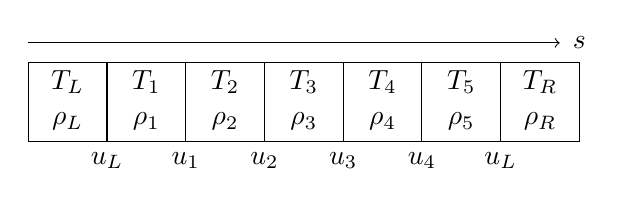
\begin{tikzpicture}
						\draw [->] (0,5/4) -- (6.75,5/4);
						\node at (7,5/4) {$s$};
					
						\draw[black](0,0) rectangle(1,1);
						\draw[black](1,0) rectangle(1,1);
						\draw[black](2,0) rectangle(1,1);
						\draw[black](3,0) rectangle(1,1);
						\draw[black](4,0) rectangle(1,1);
						\draw[black](5,0) rectangle(1,1);
						\draw[black](6,0) rectangle(1,1);
						\draw[black](7,0) rectangle(1,1);
						
						\node at (1/2,1/4) {$\rho_L$};
						\node at (3/2,1/4) {$\rho_1$};
						\node at (5/2,1/4) {$\rho_2$};
						\node at (7/2,1/4) {$\rho_3$};
						\node at (9/2,1/4) {$\rho_4$};
						\node at (11/2,1/4) {$\rho_5$};
						\node at (13/2,1/4) {$\rho_R$};
						
						\node at (1/2,3/4) {$T_L$};
						\node at (3/2,3/4) {$T_1$};
						\node at (5/2,3/4) {$T_2$};
						\node at (7/2,3/4) {$T_3$};
						\node at (9/2,3/4) {$T_4$};
						\node at (11/2,3/4) {$T_5$};
						\node at (13/2,3/4) {$T_R$};
						
						\node at (1,-1/4) {$u_L$};
						\node at (2,-1/4) {$u_1$};
						\node at (3,-1/4) {$u_2$};
						\node at (4,-1/4) {$u_3$};
						\node at (5,-1/4) {$u_4$};
						\node at (6,-1/4) {$u_L$};
					\end{tikzpicture}
					\caption{Visualization of the staggered grid on which dynamic quantities are evaluated. $\phi_L$ represents the value of each quantity on the left boundary while $\phi_R$ is the right boundary value. }
				\end{figure}

			
				The gas-dynamic equations form a coupled, nonlinear, second-order system of three partial differential equations, given here in the same form as \cite{2014ApJ...795...10L}.
				
				\begin{gather}
					\frac{\partial \rho}{\partial t} + \frac{\partial}{\partial s} \left( \rho u \right) = 0 \label{continuity} \\
					\rho \left( \frac{\partial u}{\partial t} + u \frac{\partial u}{\partial s} \right) = \frac{\partial p}{\partial s} + \frac{\partial}{\partial s} \left( \frac{4}{3} \mu \frac{\partial u}{\partial s} \right) \label{momentum} \\
					c_v \rho \left( \frac{\partial T}{\partial t} + u  \frac{\partial T}{\partial s} \right) = -p \frac{\partial u}{\partial s} + \frac{4}{3} \mu \left( \frac{\partial u}{\partial s} \right)^2 + \frac{\partial}{\partial s} \left( \kappa \frac{\partial T}{\partial s} \right) + \dot{Q} \label{energy}
				\end{gather}
				where Equation \ref{continuity} is known as the continuity equation, Equation \ref{momentum} is known as the momentum equation and Equation \ref{energy} is known as the energy equation. These equations will be interpreted using the finite difference scheme to construct update rules for density, velocity and temperature.
				
				To complete Equations \ref{continuity} through \ref{energy}, we need to define the pressure in terms of the ideal gas law		
				\begin{equation}
					p = \frac{k_B}{\bar{m}} \rho T \label{pressure}
				\end{equation}	
				where $k_B$ is Boltzmann's constant in erg/K and $\bar{m}$ is the mean mass per particle. In accordance with \cite{2014ApJ...795...10L} we will take this quantity to be that of a fully ionized plasma with coronal abundances, $\bar{m} = 0.593 m_p$, where $m_p$ is the proton mass in grams. Since the pressure is defined in terms of the ideal gas, we can take the specific heat to be that of a monotonic ideal gas,		
				\begin{equation}
					c_v = \frac{3}{2} \frac{k_B}{\bar{m}}. \label{specific_heat}
				\end{equation}		
				For the thermal conductivity, we take the classic Spitzer form, given by \cite{1965RvPP....1..205B}
				\begin{equation}
					\kappa = \kappa_0 T^{5/2} \label{thermal_conductivity}
				\end{equation}
				where $\kappa_0 = 10^{-6}$ erg cm$^{-1}$ s$^{-1}$ K$^{-7/2}$. Using this form for the thermal conductivity, we can take the dynamic viscosity, $\mu$, to have the same temperature dependence
				\begin{equation}
					\mu = \text{Pr} \frac{\kappa}{c_v}.\label{viscosity}
				\end{equation}
				The dynamic viscosity is attenuated by the Prandtl number Pr. To simplify comparison with Section 3 of \cite{2014ApJ...795...10L} and to make shocks easier to resolve, we will take the value of the Prandtl number to be $\text{Pr} = 10^{-4}$, which is lower than the accepted value of $\text{Pr} = 0.012$.
				
				Equations \ref{pressure} through \ref{viscosity} are allow the continuity, momentum and energy equations to be defined completely in terms of the dependent and independent variables and known constants, with the exception of $\dot{Q}$, which will be completed in Section \ref{bc}.
				
			\subsection{Finite Difference Form}
			
				To solve Equations \ref{continuity} through \ref{energy}, we will be using the method of first-order explicit finite difference. For this technique, derivatives are found for each grid point by taking a weighted sum of of its immediate neighbors. The weights of this sum are known as a \textit{stencil}, and we will use two stencils to solve the gas-dynamic equations, a forward-difference stencil, and a upwind-difference stencil, described below.
				
				We will define the forward difference stencil in terms of the function
				\begin{equation}
					\frac{\partial \phi}{\partial x} \cong \mathcal{D}(\Phi, X, \mathbf{i},\mathbf{\Delta}) = \frac{\Phi_{\mathbf{i} + \mathbf{\Delta}} - \Phi_{\mathbf{i}}}{X_{\mathbf{i} + \mathbf{\Delta}} - X_{\mathbf{i}}}
				\end{equation}
				Where $\Phi$ is a matrix with components $\Phi_\mathbf{i} = \Phi_{n,i}$ representing the value of some quantity $\phi$ evaluated at discrete points in space and time on a rectangular grid. $X$ is also a matrix with components $X_\mathbf{i} = X_{n,i}$, describing the location of each discrete grid point in space-time. The quantity $\mathbf{i}$ is a vector representing the current space-time index
				\begin{equation}
					\mathbf{i} = (n,i) = n \ \hat{t} + i \ \hat{x},
				\end{equation}
				where $\hat{t}$ is a unit vector along the time dimension and $\hat{x}$ is a unit vector along the space dimension. Finally the quantity $\mathbf{\Delta}$ is also an index vector, and it represents the direction of the derivative. A time derivative indicates that $\mathbf{\Delta} = \hat{t}$ and a spatial derivative is then $\mathbf{\Delta} = \hat{x}$.
				
				Next, we define the upwind difference stencil as a piecewise function
				\begin{gather}
				a(x) \frac{\partial \phi}{\partial x} \cong \mathcal{U}(\Phi, X, \mathbf{i}, \mathbf{\Delta}, A) \\		
				\mathcal{U}(\Phi, X, \mathbf{i}, \mathbf{\Delta}, A) = \begin{cases}
					A_{\mathbf{i}} \mathcal{D}(\Phi, X, \mathbf{i} - \mathbf{\Delta}, \mathbf{\Delta}),  &A_{\mathbf{i}} > 0 \\
					A_{\mathbf{i}} \mathcal{D}(\Phi, X, \mathbf{i}, \mathbf{\Delta}), &A_{\mathbf{i}} < 0 \\
				\end{cases}.
				\end{gather}
				The upwind stencil is used in the case where the derivative of a quantity evaluated on an edge of a cell needs to be determined at the center of a cell (or vis-versa). The naive choice for this situation, a center difference stencil would be sub-optimal here, as it would lead to the checkerboard instability, discussed above.
				
				To further aid our dealings with the staggered grid, we will also define the interpolation function, which uses linear interpolation to find the value of some quantity midway between two grid points
				\begin{equation}
					\phi \cong \mathcal{L}(\Phi, \mathbf{i},\mathbf{\Delta}) = \frac{\Phi_{\mathbf{i} + \mathbf{\Delta}} + \Phi_{\mathbf{i}}}{2}.
				\end{equation}
				This function will be used any time we need to switch the evaluation of any quantity from center to edge or edge to center.
				
				For readability in the following sections, we will define the specific derivatives
				\begin{gather}
					\mathcal{D}_t(\Phi_{\mathbf{i}}) = \mathcal{D}(\Phi, X, \mathbf{i},\hat{t}) \\
					\mathcal{D}_s(\Phi_{\mathbf{i}}) = \mathcal{D}(\Phi, X, \mathbf{i},\hat{x}) \\
					\mathcal{U}_t(\Phi_{\mathbf{i}}, A_{\mathbf{i}}) = \mathcal{U}(\Phi, X, \mathbf{i},\hat{t}, A) \\
					\mathcal{U}_s(\Phi_{\mathbf{i}}, A_{\mathbf{i}}) = \mathcal{U}(\Phi, X, \mathbf{i},\hat{x}, A) \\
					\mathcal{L}(\Phi_{\mathbf{i}}) = \mathcal{D}(\Phi, \mathbf{i},\hat{x})
				\end{gather}
				Using these definitions, we can now define the gas-dynamic equations in finite-difference form.
			
				\subsubsection{Continuity Equation}
				
					The first equation we will discretize is the continuity equation,
					\begin{equation}
						\frac{\partial \rho}{\partial t} + \frac{\partial}{\partial s} \left( \rho u \right) = 0 \nonumber
					\end{equation}
					This form is slightly opaque, so we expand using the chain rule and inspect to see which terms need to modified to be evaulated at the correct location.
					\begin{equation}
						\Rightarrow \underbrace{\frac{\partial \rho}{\partial t}}_\text{center} = \underbrace{-\rho \frac{\partial u}{\partial s}}_\text{center} \underbrace{- u \frac{\partial \rho}{\partial s}}_\text{edge} \label{cont2}
					\end{equation}
					In the above Equation, we can see that term $\ref{cont2}.1 = \partial \rho / \partial t$ is expressed in the center, so all the terms on the LHS must also be evaluated in the center. In term \ref{cont2}.2, $\rho$ is expressed at the center, while the derivative of $u$ is also expressed at the center. For these first two terms we can simply use the $\mathcal{D}$ function to evaluate the derivatives.
					
					In term \ref{cont2}.3 however, both quantities are expressed at the wrong location, at the edge. Here, we use the $\mathcal{L}$ function to evaluate $u$ at the correct location, and then plug the result into the upwind function $\mathcal{U}$. Putting it all together gives
					\begin{align}
						\ref{cont2}.1 &= \frac{\partial \rho}{\partial s} \nonumber \\ &\rightarrow \mathcal{D}_t(\rho_{\mathbf{i}}) \\
						\ref{cont2}.2 &= -\rho \frac{\partial u}{\partial s} \nonumber \\ &\rightarrow - \rho_{\mathbf{i}} \: \mathcal{D}_s(u_{\mathbf{i}}) \\
						\ref{cont2}.3 &= -u \frac{\partial \rho}{\partial s} \nonumber \\ &\rightarrow - \mathcal{U}_s( \rho_{\mathbf{i}}, \mathcal{L}(u_{\mathbf{i}}))
					\end{align}
				
				\subsubsection{Momentum Equation}
					Next, we will discretize the momentum equation, given by
					\begin{equation}
						\rho \left( \frac{\partial u}{\partial t} + u \frac{\partial u}{\partial s} \right) = \frac{\partial p}{\partial s} + \frac{\partial}{\partial s} \left( \frac{4}{3} \mu \frac{\partial u}{\partial s} \right) \nonumber
					\end{equation}
					Rewriting in the same manner as the continuity equation gives
					\begin{equation}
						\frac{\partial u}{\partial t} = -u \frac{\partial u}{\partial s} - \frac{1}{\rho} \frac{\partial p}{\partial s} + \frac{4 \mu_0}{3} \frac{1}{\rho} \frac{\partial}{\partial s} \left( T^{5/2} \frac{\partial u}{\partial s} \right) \label{mom2}
					\end{equation}
					Term \ref{mom2}.1 is evaluated on the edge, so all terms on the LHS should also be evaluated at edges. Expression \ref{mom2}.2.2 is expressed on centers, so we will use an the upwind scheme on term \ref{mom2}.2. All factors of $1/\rho$ are expressed on centers, so we will use the interpolation function to evaluate those factors at the correct location. All together then, we have
					\begin{align}
						\ref{mom2}.1 &= \frac{\partial u}{\partial t} \nonumber \\ &\rightarrow \mathcal{D}_t(u_{\mathbf{i}}), \\
						\ref{mom2}.2 &= -u \frac{\partial u}{\partial s} \nonumber \\ &\rightarrow - \mathcal{U}_s(u_{\mathbf{i}}, u_{\mathbf{i}}), \\
						\ref{mom2}.3 &= -\frac{1}{\rho} \frac{\partial p}{\partial s} \nonumber \\ &\rightarrow \frac{k_B / \bar{m}}{\mathcal{L}(\rho_{\mathbf{i}})} \mathcal{D}_s(\rho_{\mathbf{i}} T_{\mathbf{i}}), \\
						\ref{mom2}.4 &=  \frac{4 \mu_0}{3} \frac{1}{\rho} \frac{\partial}{\partial s} \left( T^{5/2} \frac{\partial u}{\partial s} \right) \nonumber \\ &\rightarrow  \frac{4 \mu_0}{3}  \frac{1}{\mathcal{L}(\rho_{\mathbf{i}})} \mathcal{D}_s\left( T_{\mathbf{i}}^{5/2} \mathcal{D}_s(u_{\mathbf{i}}) \right).
					\end{align}
					
				\subsubsection{Energy Equation}
				
					Finally, dropping the constant $\dot{Q}$, we have the energy equation
					\begin{equation}
						c_v \rho \left( \frac{\partial T}{\partial t} + u  \frac{\partial T}{\partial s} \right) = -p \frac{\partial u}{\partial s} + \frac{4}{3} \mu \left( \frac{\partial u}{\partial s} \right)^2 + \frac{\partial}{\partial s} \left( \kappa \frac{\partial T}{\partial s} \right) \nonumber
					\end{equation}
					Rearranging terms gives
					\begin{equation}
						\begin{split}
						\frac{\partial T}{\partial t} = -u \frac{\partial T}{\partial s} - \frac{1}{c_v} \frac{p}{\rho} \frac{\partial u}{\partial s} + \frac{4 \mu_0}{3 c_v} \frac{T^{5/2}}{\rho} \left(\frac{\partial u}{\partial s}\right)^2 \\ + \frac{\kappa_0}{c_v} \frac{1}{\rho} \frac{\partial}{\partial s} \left( T^{5/2} \frac{\partial T}{\partial s} \right) 
						\end{split}
						\label{e2}
					\end{equation}
					For this equation, Term \ref{e2}.1 is expressed on centers. However, term \ref{e2}.2 is expressed on edges, so we will again use the upwind method to deal with this derivative. The only other troubling part of Equation \ref{e2} is the factor \ref{e2}.5.3.1.1 = $T^{5/2}$ which is expressed on centers. We will use the linear interpolation function to evaluate this term on edges, to make ensure that the expression \ref{e2}.5.3 is evaluated on centers. Under the finite difference scheme, the energy equation becomes
					\begin{align}
						\ref{e2}.1 &= \frac{\partial T}{\partial t} \nonumber \\ &\rightarrow \mathcal{D}_t(T_{\mathbf{i}}) \\
						\ref{e2}.2 &= -u \frac{\partial T}{\partial s} \nonumber \\ &\rightarrow - \mathcal{U}_s(T_{\mathbf{i}}, \mathcal{L}(u_{\mathbf{i} - \hat{x}})) \\
						\ref{e2}.3 &= - \frac{1}{c_v} \frac{p}{\rho} \frac{\partial u}{\partial s} \nonumber \\ &\rightarrow - \frac{1}{c_v} \frac{p_{\mathbf{i}}}{\rho_{\mathbf{i}}} \mathcal{D}_s(u_{\mathbf{i} - \hat{x}}) \\
						\ref{e2}.4 &= \frac{4 \mu_0}{3 c_v} \frac{T^{5/2}}{\rho} \left(\frac{\partial u}{\partial s}\right)^2 \nonumber \\ &\rightarrow \frac{4 \mu_0}{3 c_v} \frac{T_{\mathbf{i}}^{5/2}}{\rho_{\mathbf{i}}} \left[ \mathcal{D}_s(u_{\mathbf{i} - \hat{x}}) \right]^2 \\
						\ref{e2}.5 &= \frac{\kappa_0}{c_v} \frac{1}{\rho} \frac{\partial}{\partial s} \left( T^{5/2} \frac{\partial T}{\partial s} \right) \nonumber \\ &\rightarrow \frac{\kappa_0}{c_v} \frac{1}{\rho_{\mathbf{i}}} \mathcal{D}_s \left( \mathcal{L}(T_{\mathbf{i}}^{5/2}) \mathcal{D}_s(T_{\mathbf{i}}) \right)
					\end{align}
					
					Putting all of these equations together gives us the update rules for density, velocity and temperature.
		\subsection{Boundary Conditions} \label{bc}
			\subsubsection{Temporal Conditions}	\label{time_bc}
				Since the loop starts in equilibrium and gravity is neglected, we take the initial pressure to be constant across the entire spatial extent of the loop. The equilibrium condition also tells us that the initial velocity is zero across the entire loop.
				
				The initial temperature is defined using the equilibrium heating function
				\begin{equation}
					H_\text{eq} = A\left[ S(s - \Delta_\text{tr}) - S(s) + S(L - \Delta_\text{tr} - s) - S(L-s) \right] \nonumber
				\end{equation}
				where $S(x)$ is known as the shape function and is defined by
				\begin{equation}
					S(x) = \begin{cases}
						1 - (x/w - 1)^2, \quad &0 < x < 2w \\
						0, &\text{otherwise}
					\end{cases}.
				\end{equation}
				Here, $\Delta_\text{tr}$ is the width of the transition region, $L$ is the length of the loop, and $w$ is the characteristic width of the shape function. Using this equilibrium heating condition we can solve for the initial temperature distribution using the following expression provided by \cite{2014ApJ...795...10L}.
				\begin{equation}
					T^{7/2}(s) = T_\text{chr} - \frac{7}{2} \kappa_0^{-1} \int^s ds' \int^{s'} ds'' H_\text{eq}(s'')
				\end{equation}
				The above expression is usually solved numerically, for this work we solved it analytically using Mathematica.
			\subsubsection{Spatial Conditions}	\label{space_bc}
				For the spatial boundary conditions, we will take Dirichlet boundary conditions for all three quantities: density, velocity and temperature. These quantities will be held to their initial values on the edge of the grid.
				
		\subsection{Flare Heating}
			
			The flare heating is a constant function given by \cite{2014ApJ...795...10L}
			\begin{equation}
				H_\text{fl}(s) = \begin{cases}
					\frac{F}{\Delta_\text{fl}/2}, \quad &|s - L/2| < \Delta_\text{tr}/2 \\
					0, &\text{otherwise}
				\end{cases},
			\end{equation}
			where $\Delta_\text{fl}$ is the width of the flare heating function and $F$ is the total energy flux delivered to the loop.
			Using this expression, we can write $\dot{Q}$ as a sum of the equilibrium heating function and the flare heating function.
			\begin{equation}
				\dot{Q}(s) = H_\text{eq}(s) + H_\text{fl}(s)
			\end{equation}
			With this function in hand, we have all the pieces we need to start running some simulations.
			
	\section{Results}
	
		Using the information detailed in the previous sections, we developed a computer program to calculate the results of our finite difference calculations. The results below are run using the same parameters as those in \cite{2014ApJ...795...10L} Section 3.
	
		\begin{figure}[H]
			\centering
			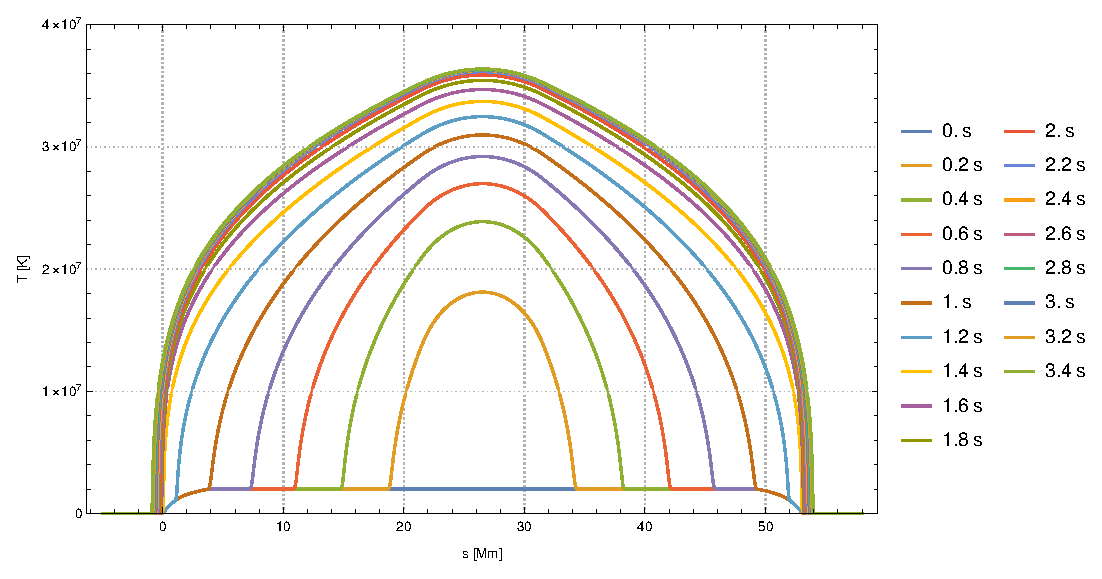
\includegraphics[width=0.5\textwidth]{figures/temp_vs_time}
			\caption{Temperature across the loop plotted at different times}
		\end{figure}
		\begin{figure}[H]
			\centering
			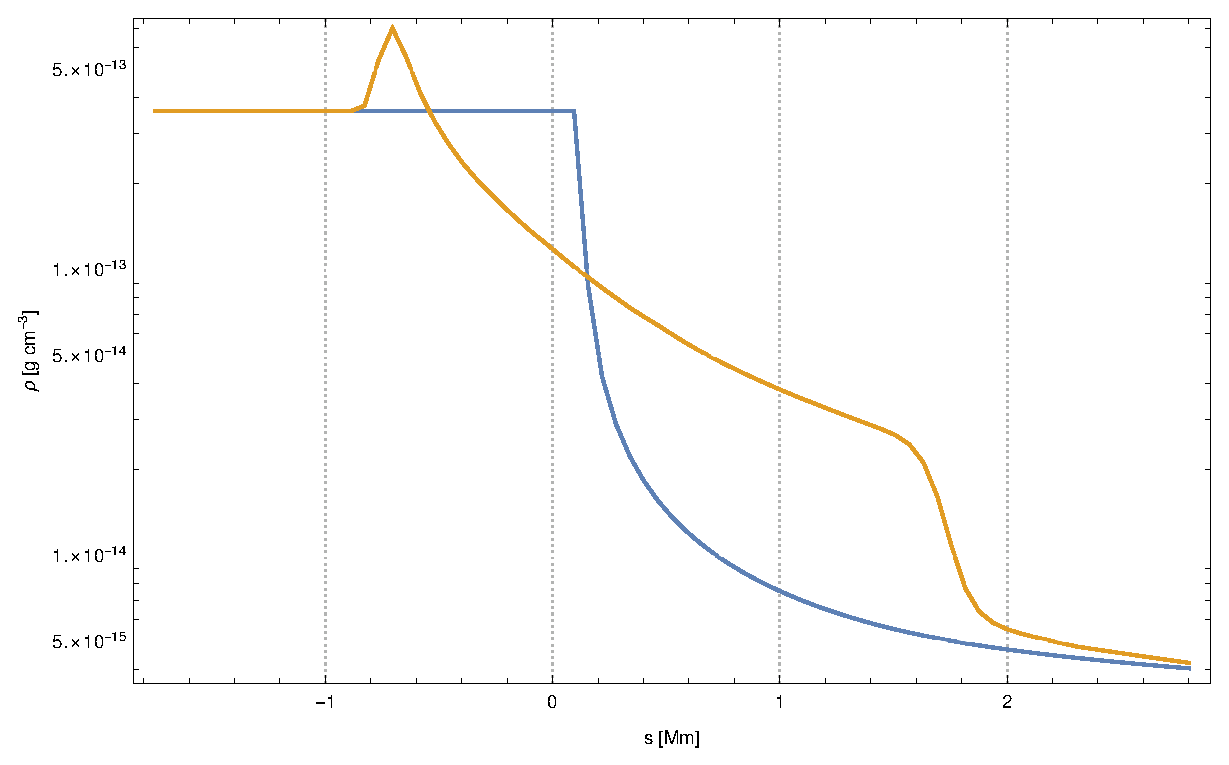
\includegraphics[width=0.5\textwidth]{figures/rho_vs_s}
			\caption{Density vs. space at $t=0$s (blue) and $t=3.5$s (orange)}
		\end{figure}
		\begin{figure}[H]
			\centering
			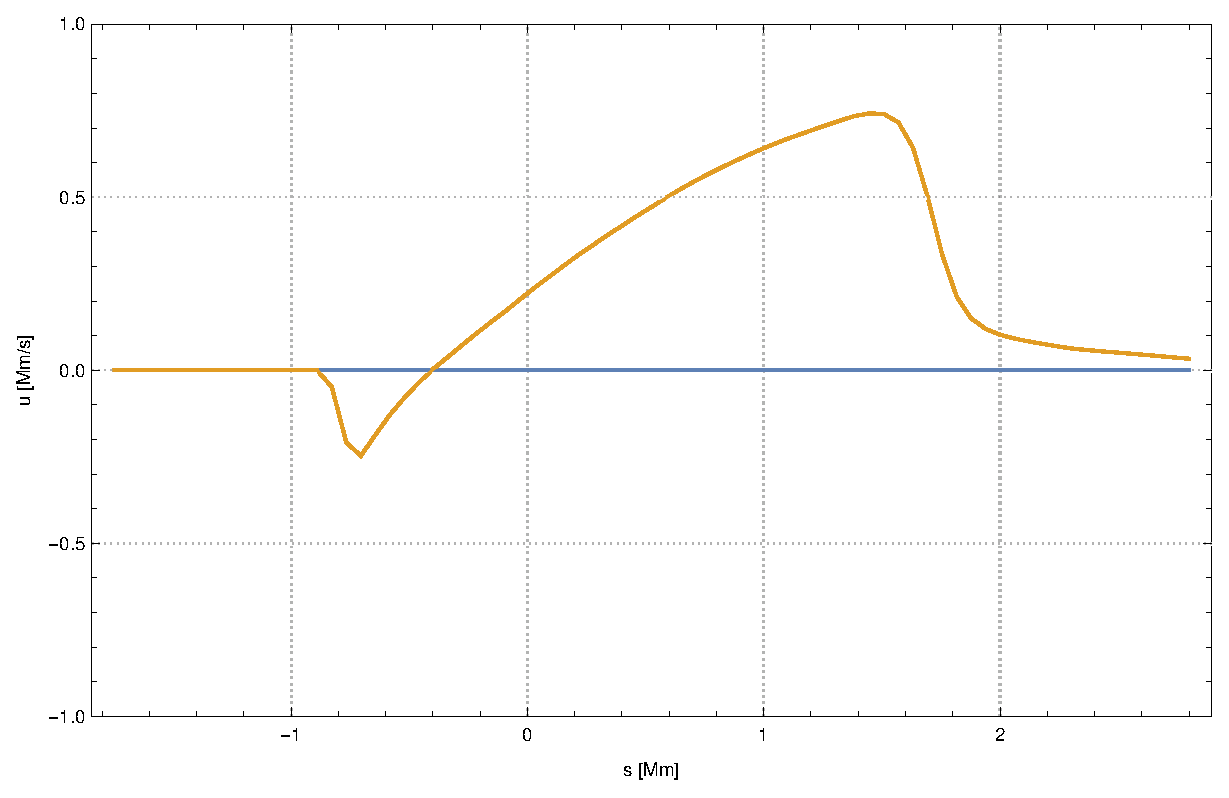
\includegraphics[width=0.5\textwidth]{figures/vel_vs_s}
			\caption{Velocity vs. space at $t=0$s (blue) and $t=3.5$s (orange)}
		\end{figure}
		\begin{figure}[H]
			\centering
			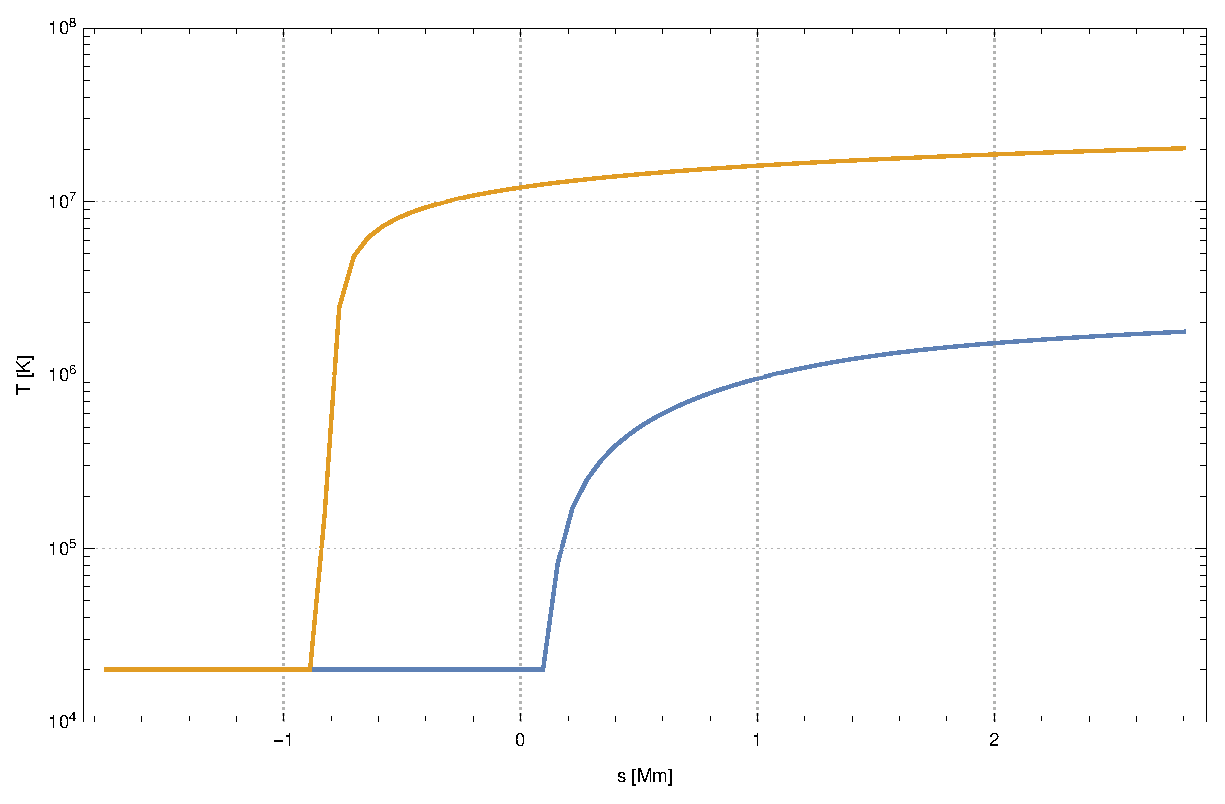
\includegraphics[width=0.5\textwidth]{figures/T_vs_s}
			\caption{Temperature vs. space at $t=0$s (blue) and $t=3.5$s (orange)}
		\end{figure}
		
		Comparing to Section 3 of \cite{2014ApJ...795...10L}, we notice that the condensation shock has not propogated as far into the chromosphere, this is possibly caused by the fact that we used a constant grid, rather than the adaptive grid used in \cite{2014ApJ...795...10L}. The lower resolution of the constant grid prevents our simulation from resolving the point correctly.
		
		Otherwise, the results obtained here seem to match pretty well to the results obtained by Longcope, the mmaximum temperature is similar, and the thermal conduction front has propagated the same amount into the chromosphere.
	
	\section{Conclusion}
	
		We have detailed the steps required to solve the gas-dynamic equations in a flare loop using the method of explicit finite difference. Future studies will continue to verify this code against other simulations performed in \cite{2014ApJ...795...10L}, and also expand this code to include more terms, implicit solvers and GPU acceleration.

	\bibliographystyle{apj}
	\bibliography{sources}
	
\end{document}